\section*{Introduction}
Today we begin looking at insects that exhibit \latinword{holometabolous} development, sometimes referred to as complete development or complete metamorphosis. The insect orders in the following chapters are classified in a higher-level taxon named, appropriately enough, \textbf{Holometabola}. The immature stage (\latinword{larva}) is quite different, usually, from the \latinword{imago} (adult), and the transition to adulthood takes place in a stage we refer to as the \latinword{pupa}. 

\section{Larvae}
% https://doi-org.ezaccess.libraries.psu.edu/10.1016/B978-0-12-374144-8.00157-0
We will examine specimens of different types of larvae, to get a sense of their adaptations and how much they differ from adults of the same species. Larvae are frequently the life stage of consequence, as the form that infests our produce and stored products, the form that helps us determine time of death in forensic situations, the form that tells us about water quality, \textit{etc}. In that light, we will spend some time observing some diagnostic traits, including \latinword{chaetotaxy}.

\subsection{Campodeiform}
\noindent{}\textit{Basic form:} Habitus (figure \ref{fig:campodeiform1}) superficially similar to campodeid diplurans (figure \ref{fig:campodeidhab}), with well-developed legs and often with relatively long antennae and cerci. These larvae are highly mobile and usually live as predators.\vspace{3mm}

\noindent{}\textit{Example taxa:} Neuropterida, Carabidae (Coleoptera)\vspace{3mm}

\begin{figure}[ht!]
  \centering
    \includegraphics[width=0.8\textwidth]{larvae/campodeiform1}
  \caption{Campodeiform larva \citep[modified from][Plate XV]{bhlitem36654Larvae}}
  \label{fig:campodeiform1}
\end{figure}

\subsection{Elateriform} 
\noindent{}\textit{Basic form:} Habitus almost worm-like and cylindrical, with short legs and usually with a somewhat sclerotized body. These larvae, sometimes called ``wireworms'', usually live as saprophages.\vspace{3mm}

\noindent{}\textit{Example taxa:} Elateridae, some Tenebrionidae (Coleoptera)\vspace{3mm}

\begin{figure}[ht!]
  \centering
    \includegraphics[width=0.8\textwidth]{larvae/elateriform1}
  \caption{Elateriform larva \citep[modified from][Plate X]{bhlitem36654Larvae}}
  \label{fig:elateriform1}
\end{figure}

\subsection{Scarabaeiform}% https://flic.kr/p/2kLeCo8
\noindent{}\textit{Basic form:} Habitus usually C-shaped, with a heavily-sclerotized heads and well-developed legs. Despite the well-developed legs these larvae are not very quick. These larvae usually live as saprophages.\vspace{3mm}

\noindent{}\textit{Example taxa:} Scarabaeidae, Lucanidae (Coleoptera)\vspace{3mm}

\begin{figure}[ht!]
    \centering
    \begin{subfigure}[ht!]{0.38\textwidth}
      \centering
        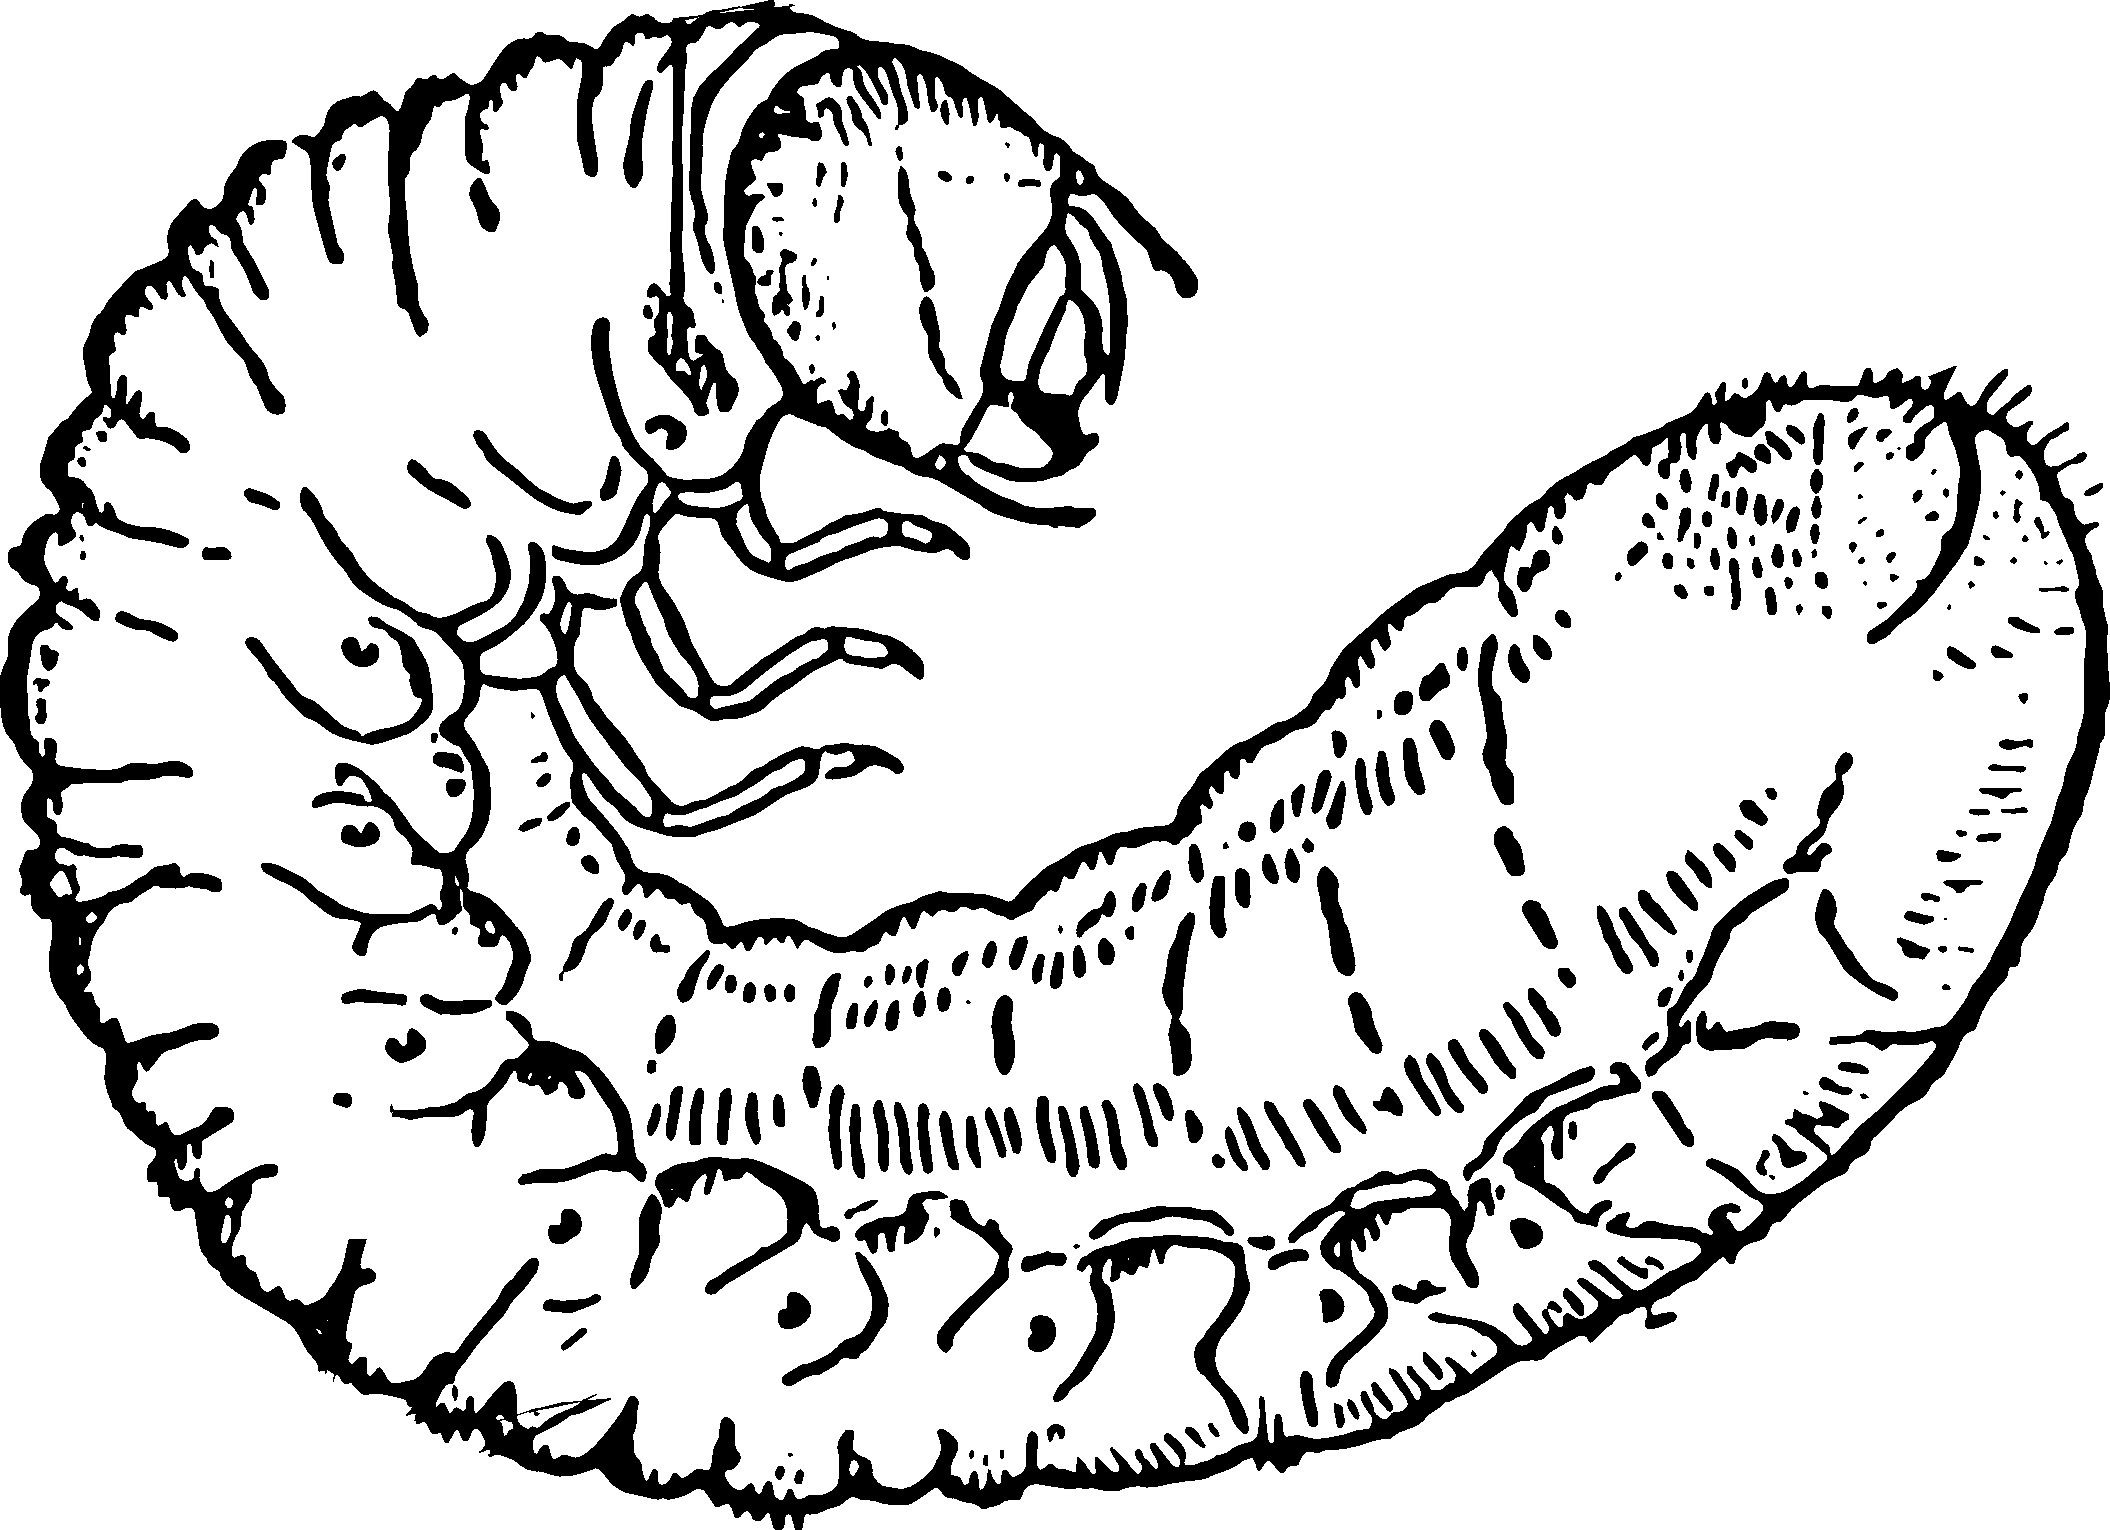
\includegraphics[width=\textwidth]{larvae/scarabaeiform1}
        \caption{scarabaeiform}
        \label{fig:scarabaeiform1}
    \end{subfigure}
    \hfill
    \begin{subfigure}[ht!]{0.48\textwidth}
        \includegraphics[width=\textwidth]{larvae/onisciform1}
        \caption{onisciform}
        \label{fig:onisciform1}
    \end{subfigure}
    \caption{\textbf{(a)} Scarabaeiform larva \citep[redrawn from][Fig. 1A]{bhlitem130205scarab}; \textbf{(b)} onisciform larva \citep[modified from][Plate IX]{bhlitem36654Larvae}}\label{fig:larvae123}
\end{figure}

\subsection{Onisciform} 
\noindent{}\textit{Basic form:} Habitus flattened and broad, often referred to as ``woodlouse-like''.\vspace{3mm}

\noindent{}\textit{Example taxa:} Psephenidae, Lampyridae, Lycidae (Coleoptera), and some Lepidoptera\vspace{3mm}

\subsection{Eruciform}% https://flic.kr/p/2kEAN6m
\noindent{}\textit{Basic form:} Habitus tube-like, with heavily sclerotized head capsule, flexible cuticle, and usually with \latinword{prolegs} present. The term is derived from the Latin words for ``caterpillar-like''. These larvae are often herbivorous.\vspace{3mm}

\noindent{}\textit{Example taxa:} Lepidoptera, non-apocritan Hymenoptera (``Symphyta'')\vspace{3mm}

\begin{figure}[ht!]
  \centering
    \reflectbox{%
      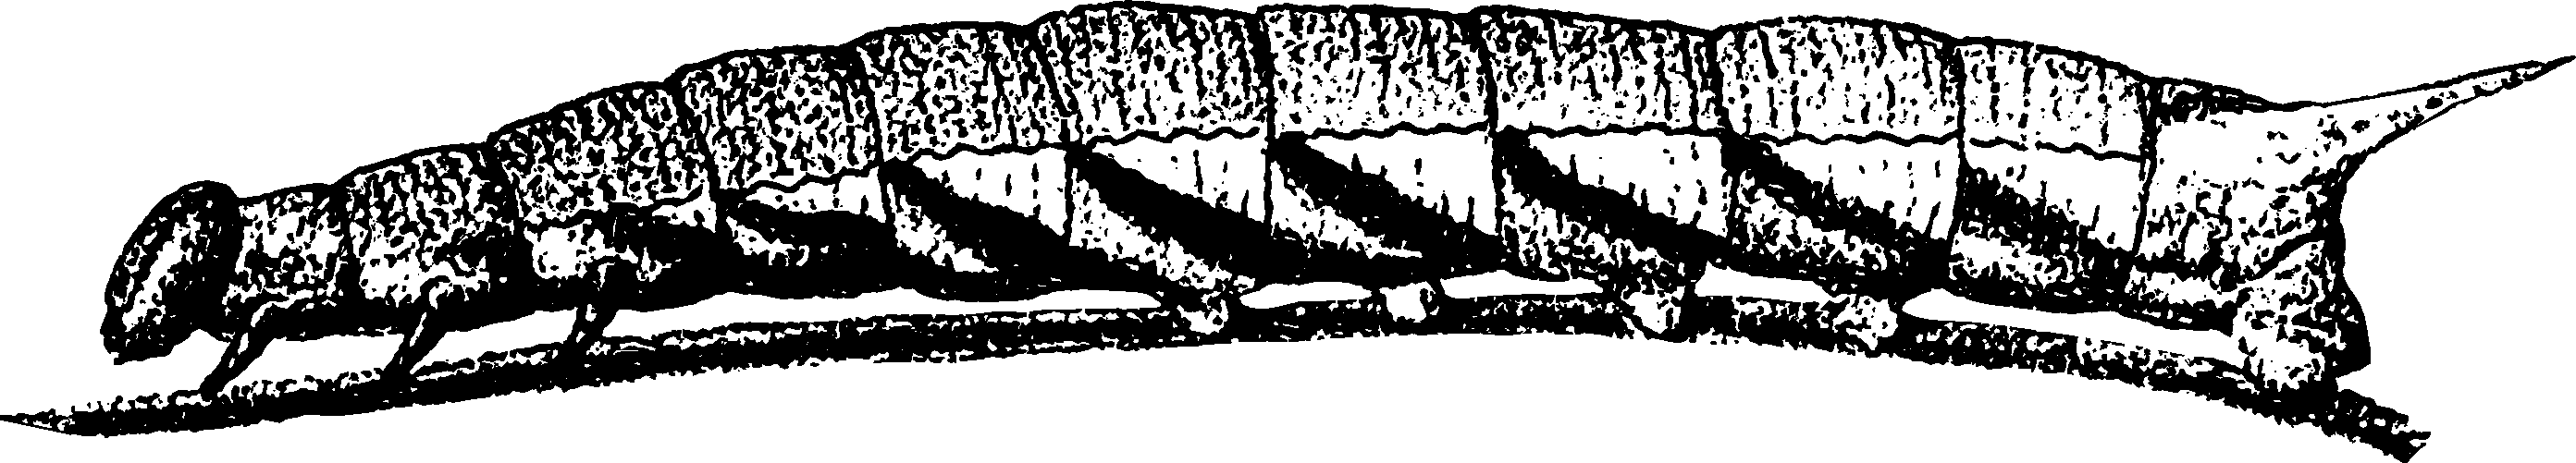
\includegraphics[width=0.8\textwidth]{larvae/eruciform1}}
  \caption{Eruciform larva \citep[redrawn from][Plate VII]{fawcett1901notes}}
  \label{fig:eruciform1}
\end{figure}

\subsection{Vermiform}
\noindent{}\textit{Basic form:} Habitus worm-like and cylindrical, legs absent, head usually indistinct.\vspace{3mm}

\noindent{}\textit{Example taxa:} Diptera\vspace{3mm}

\begin{figure}[ht!]
  \centering
    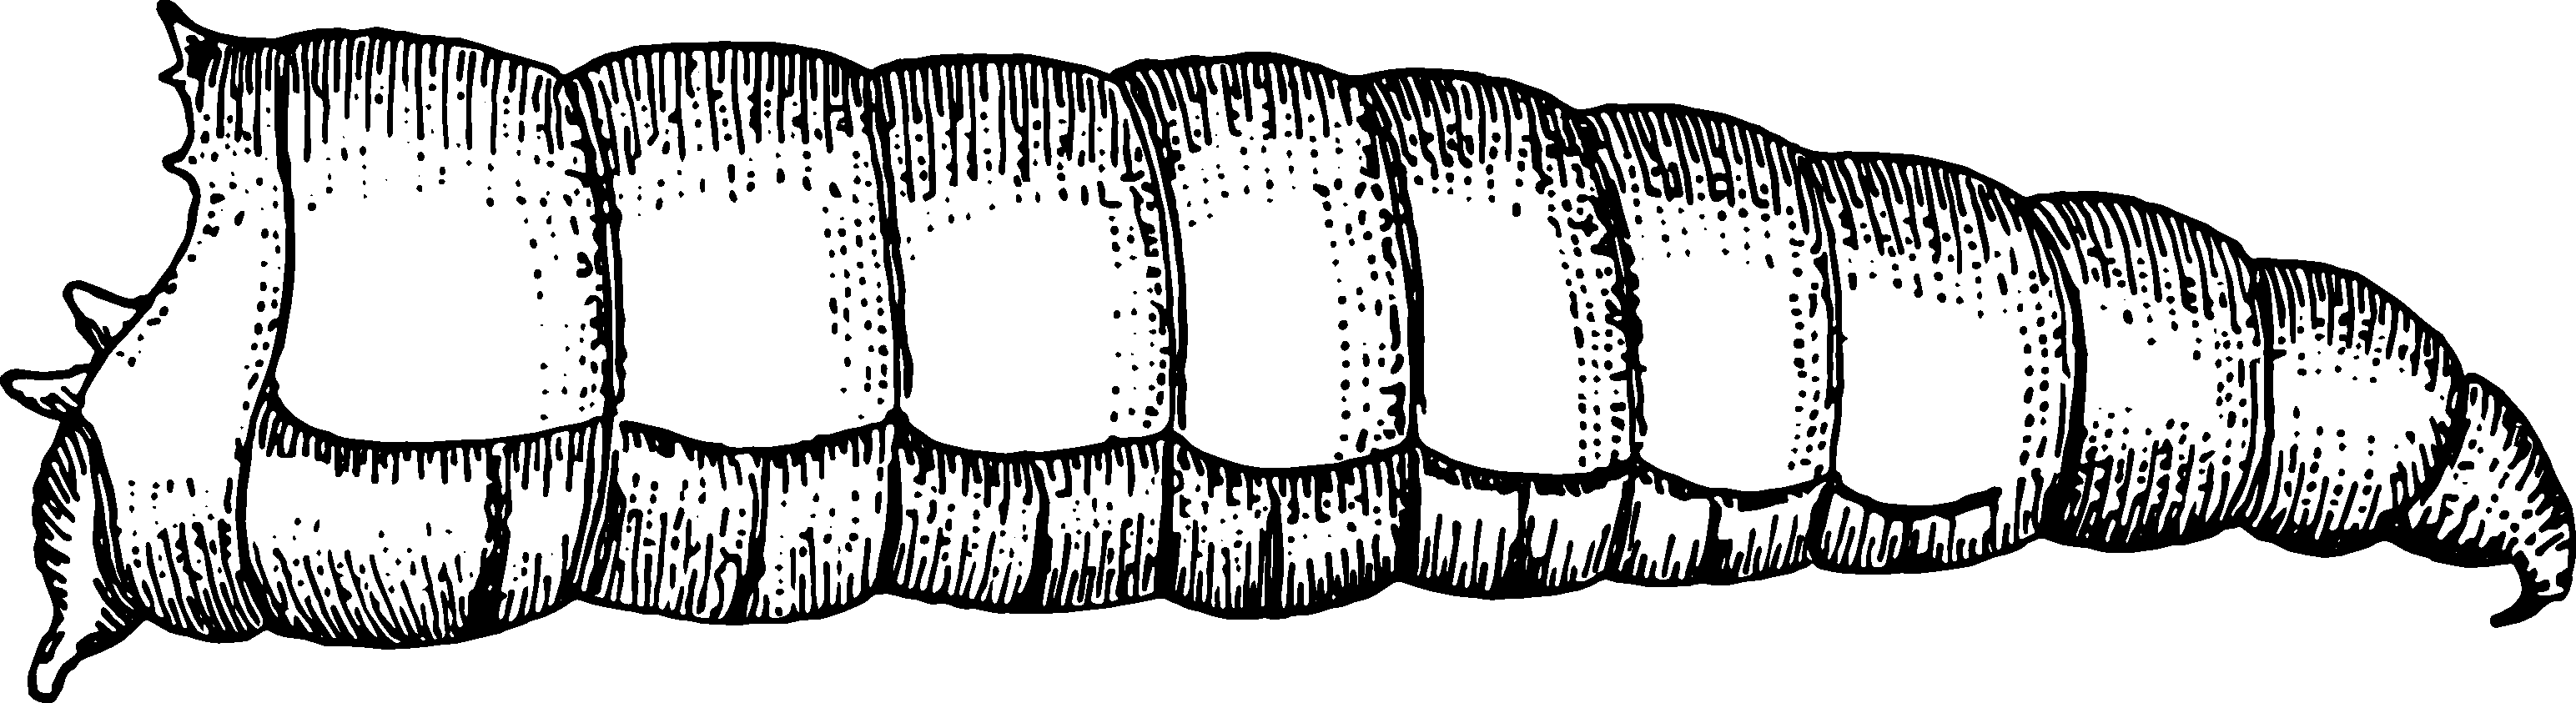
\includegraphics[width=0.55\textwidth]{larvae/vermiform1}
  \caption{Vermiform larva (maggot) \citep[redrawn from][Fig. 4a]{bhlitem92397tringulin}}
  \label{fig:triungulin}
\end{figure}

\subsection{Triungulin}
\noindent{}\textit{Basic form:} Habitus campodeiform or elateriform, usually, and often very small (1 mm or less). Name derived from claws at the apices of legs. These forms are usually adapted for grabbing onto a host and will undergo hypermetamorphosis in subsequent stages.\vspace{3mm}

\noindent{}\textit{Example taxa:} some Coleoptera (Meloidae), Strepsiptera\vspace{3mm}

\begin{figure}[ht!]
  \centering
    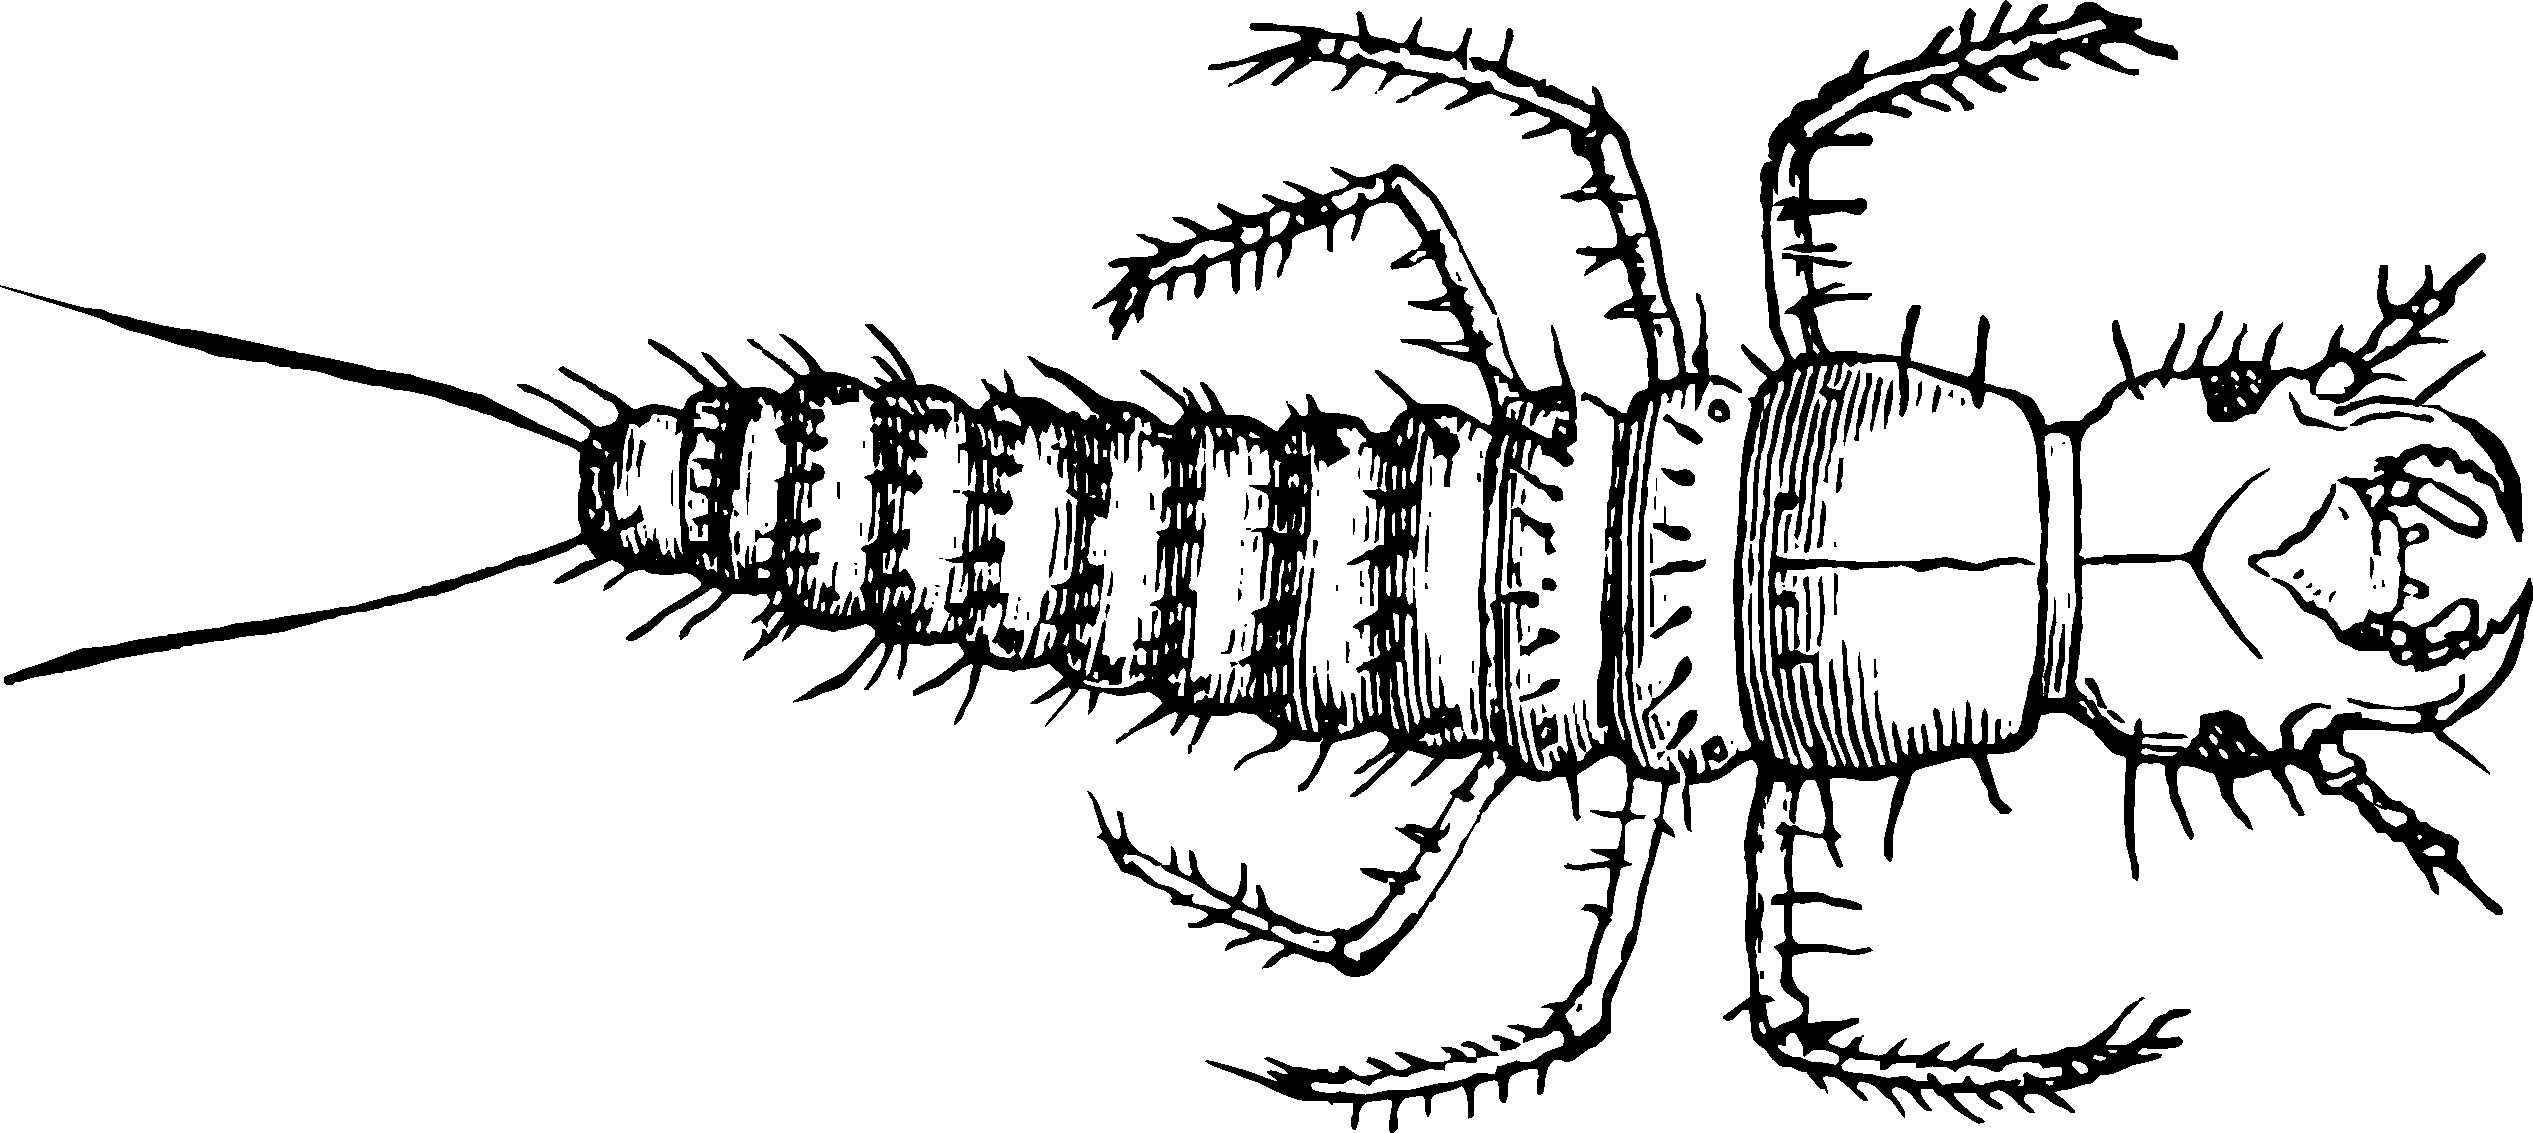
\includegraphics[width=0.12\textwidth]{larvae/triungulin}
  \caption{Triungulin (Coleoptera: Meloidae) \citep[redrawn from][Fig. 230c]{bhlitem34045maggot}}
  \label{fig:vermiform1}
\end{figure}

\begin{theo}
{}Given examples of the types of larvae above, can explain why certain parts are sclerotized, while other parts remain highly flexible? For example, why are the spiracle openings sclerotized in the scarabaeiform larvae?\vspace{3mm}

\noindent{}Are the terms above sufficient for characterizing the diversity of insect larvae? Which category describes mosquito larvae (Culicidae) in figure \ref{fig:culicidLarva}?
\end{theo}

\begin{figure}[ht!]
  \centering
    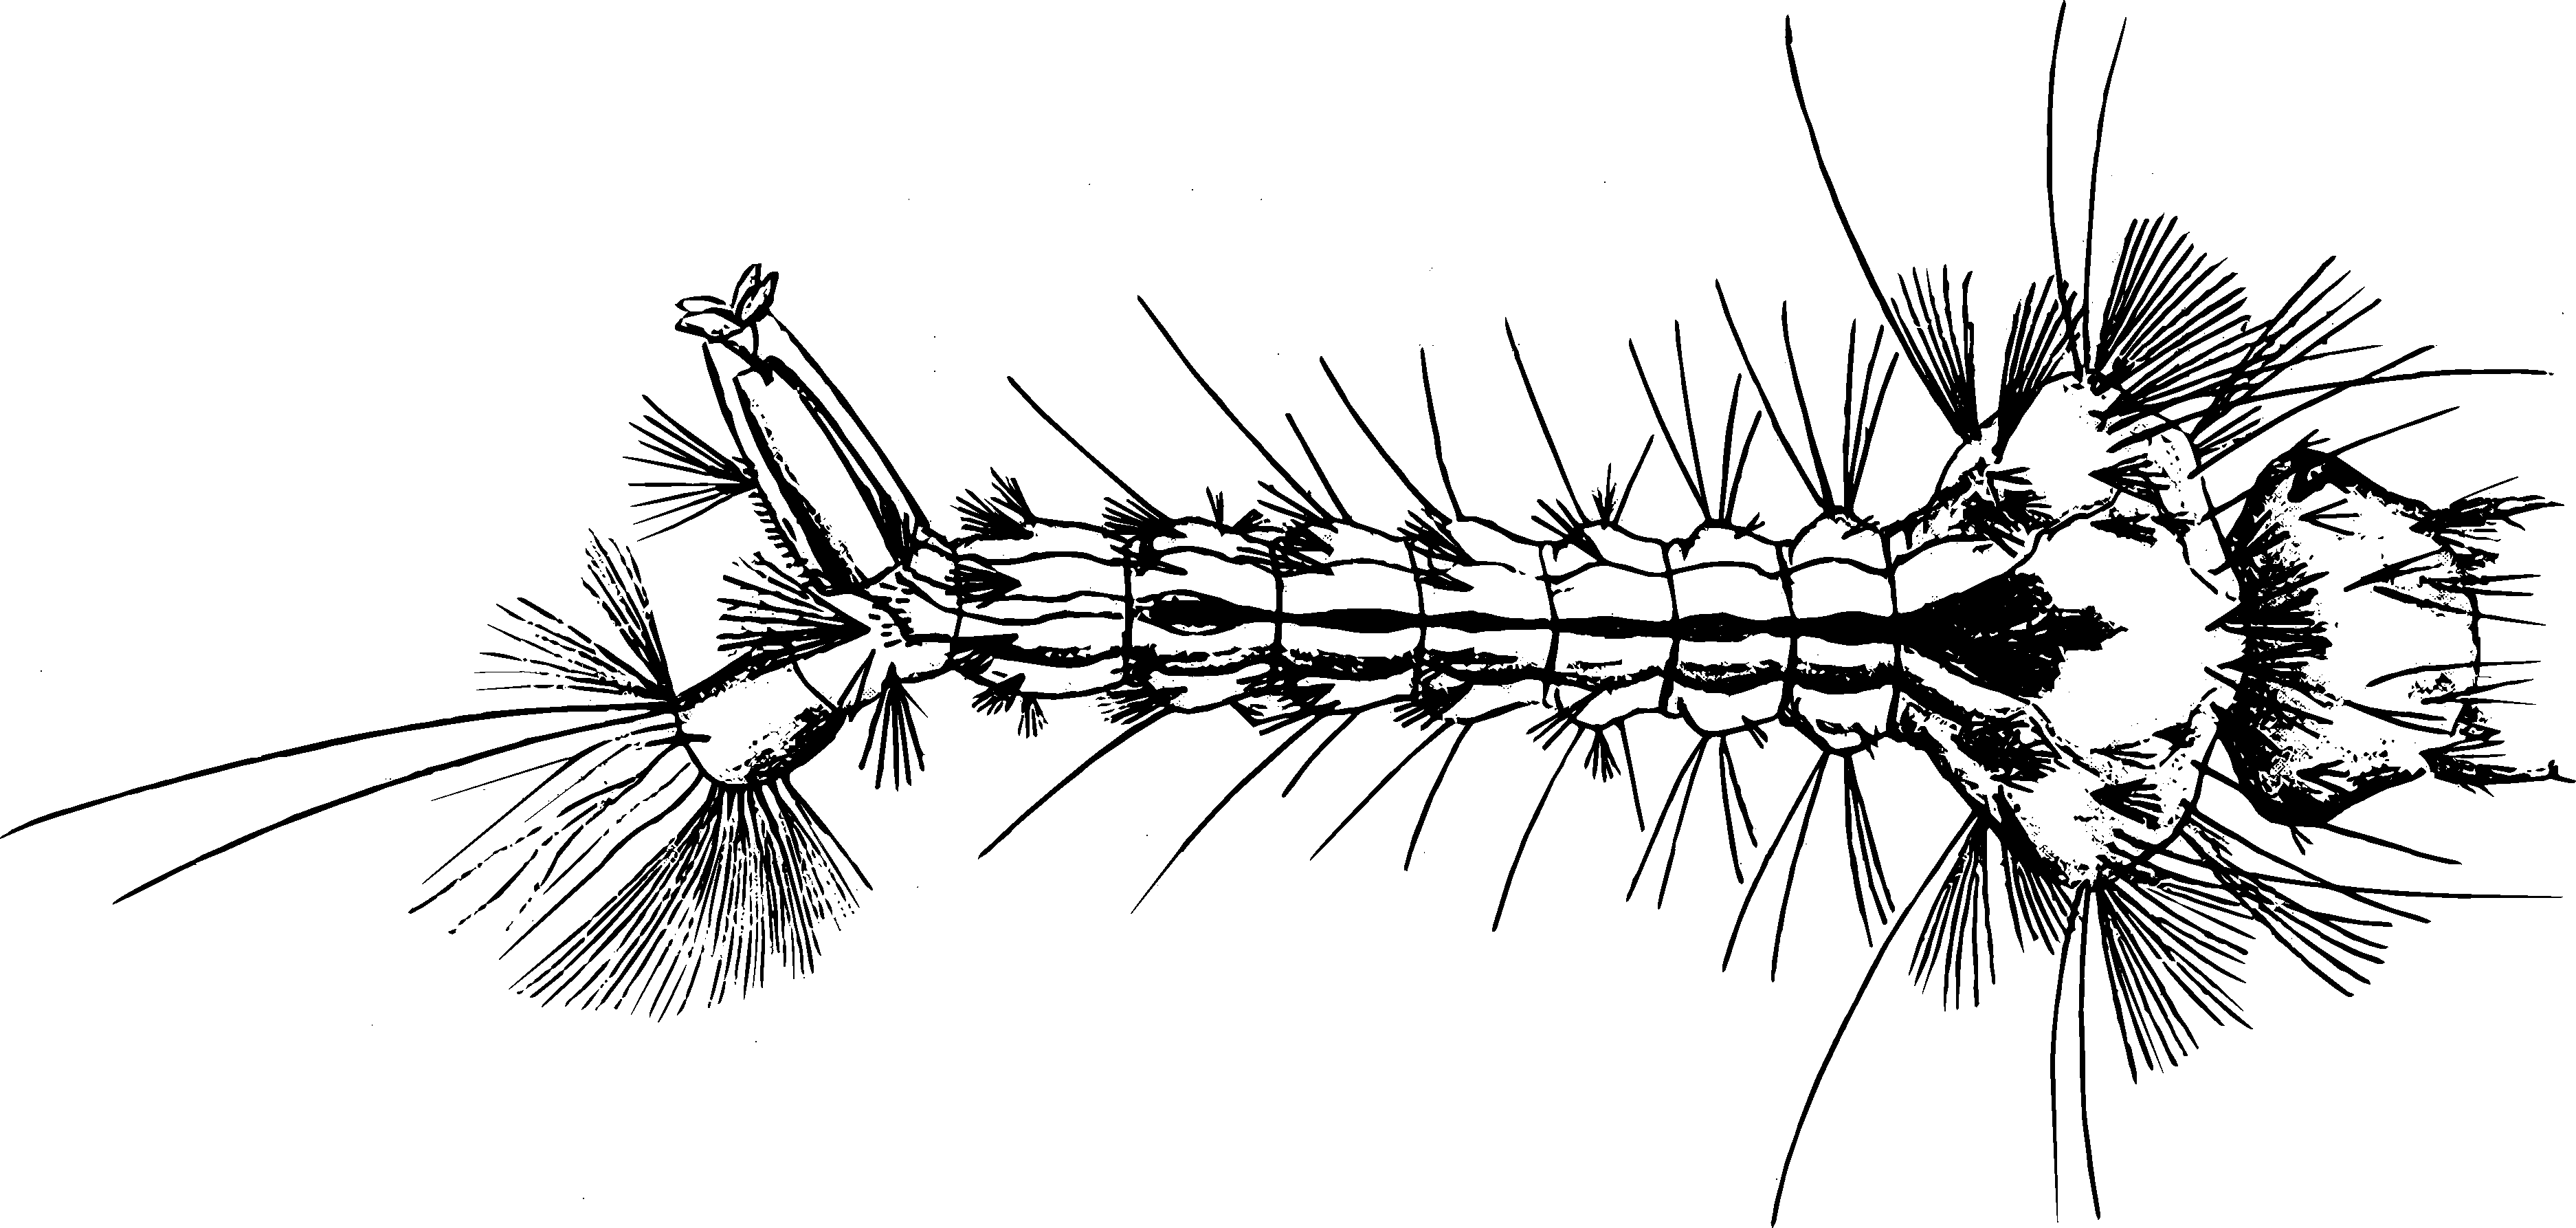
\includegraphics[width=0.7\textwidth]{larvae/culicidLarva}
  \caption{Mosquito larva (wriggler) \citep[redrawn from][Plate III]{bhlitem49255}}
  \label{fig:culicidLarva}
\end{figure}

\section{Chaetotaxy}

Insects are covered in setae, the patterns of which can be diagnostic. The naming and describing of these patterns is referred to as \latinword{chaetotaxy}, and you'll see these characters become important when we study adult Diptera. Chaetotaxy is also relevant when trying to determine larvae to family. We will examine some of these characters and learn some of the basic annotations, including, for Lepidoptera anyway:
\begin{itemize}
    \item microseta (M) - a short seta, presumed to proprioceptive
    \item pore (a) - a pit that is assumed to have some glandular function
    \item dorsal (D) - on the dorsum
    \item anterior (A) - on anterior surface of head capsule
    \item subdorsal (SD) - just lateral of the dorsal plane
    \item stemmatal (S) - near the stemmata
    \item substemmatal (SS) - ventral of most stemmata
    \item ocellar (O) - near the ocelli
    \item frons (F) - on frons
    \item adfrontal (AF) - between adfrontal suture and ecdysial line
    \item posteriodorsal (P) - on face
    \item clypeal (C) - on clypeus
    \item genal (G) - near the gena (``cheek'')
    \item lateral (L) - on the side
    \item subventral (SV) - just dorsal of the venter
    \item ventral (V) - on the venter
\end{itemize}\vfill

\begin{theo}
{}Look at the structures in figures \ref{fig:headchaeto}--\ref{fig:thoraxchaeto}. Some of the setae, microsetae, and pores are labeled. Can you annotate the remaining structures with appropriate labels? Observe the chaetotaxy exhibited by some of the available caterpillar specimens. Try sketching an abdominal segment, including the spiracle and setae you see and the pattern of the proleg crochets. The aim is not necessarily to get you to memorize these terms but to familiarize yourself with the morphology, in case you need to identify your own larvae.
\end{theo}

\begin{figure}[ht!]
    \centering
    \begin{subfigure}[ht!]{0.65\textwidth}
      \centering
        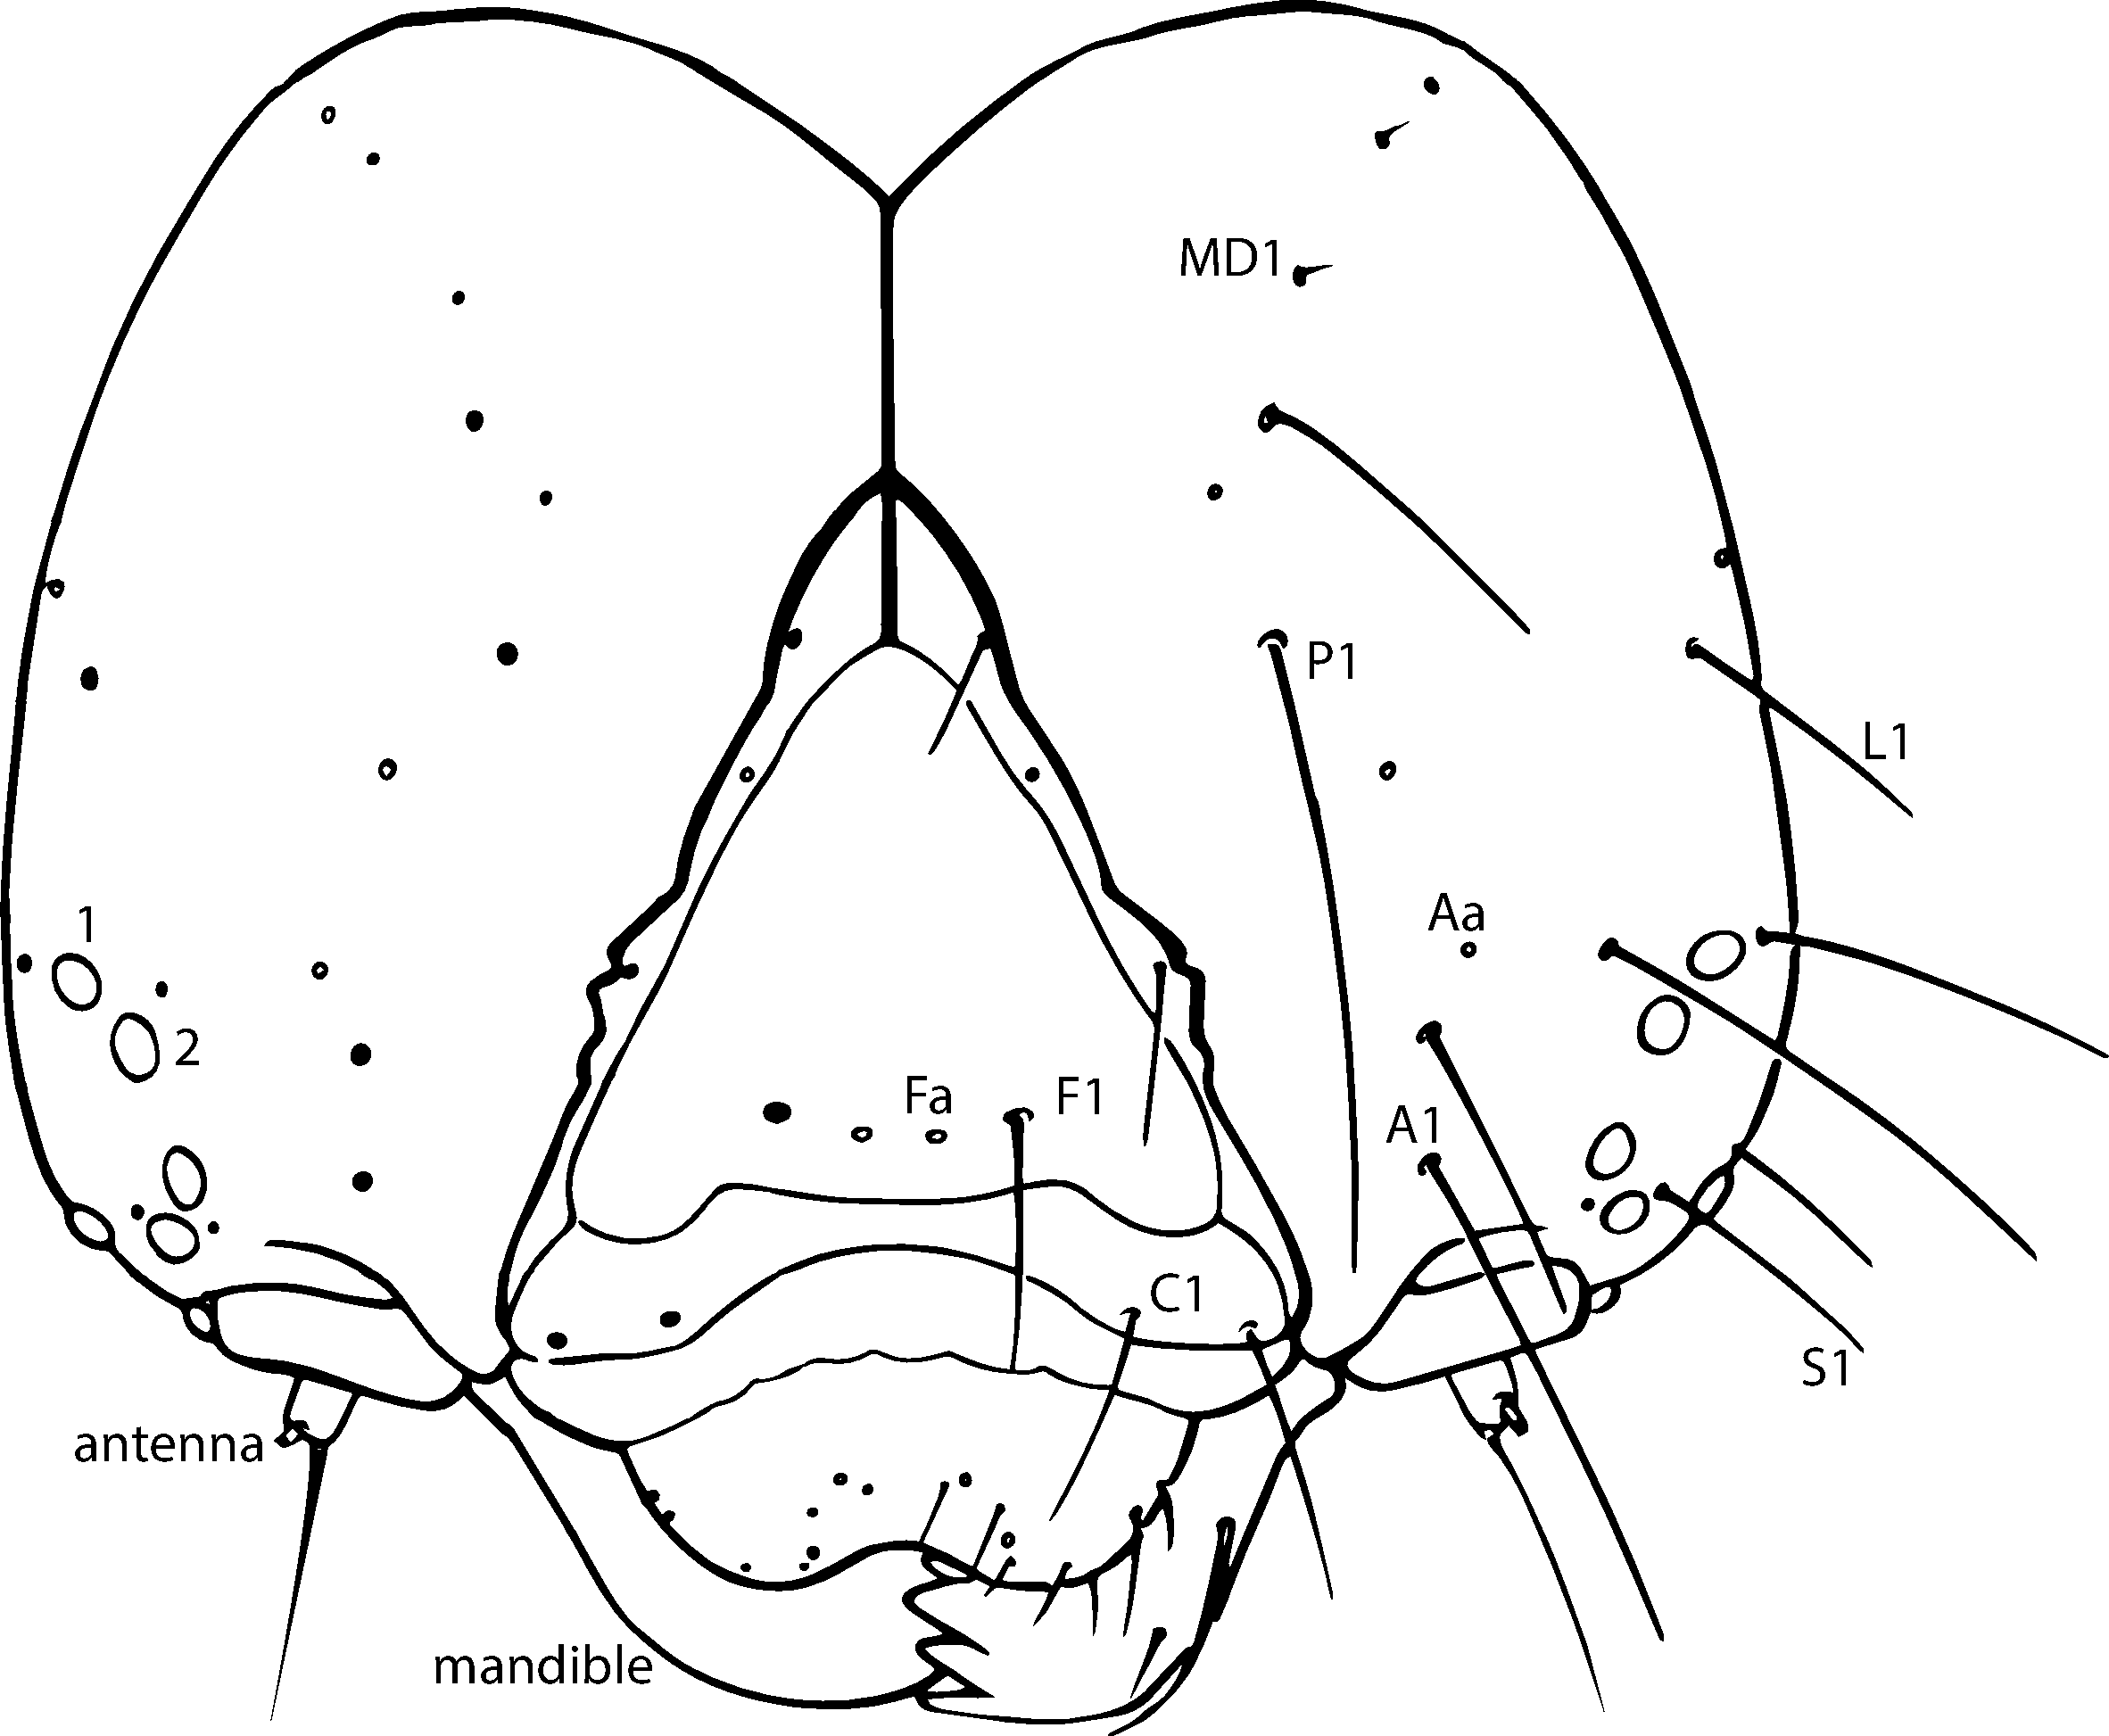
\includegraphics[width=\textwidth]{larvae/headChaeto}
        \caption{head}
        \label{fig:headchaeto}
    \end{subfigure}
    \hfill
    \begin{subfigure}[ht!]{0.25\textwidth}
        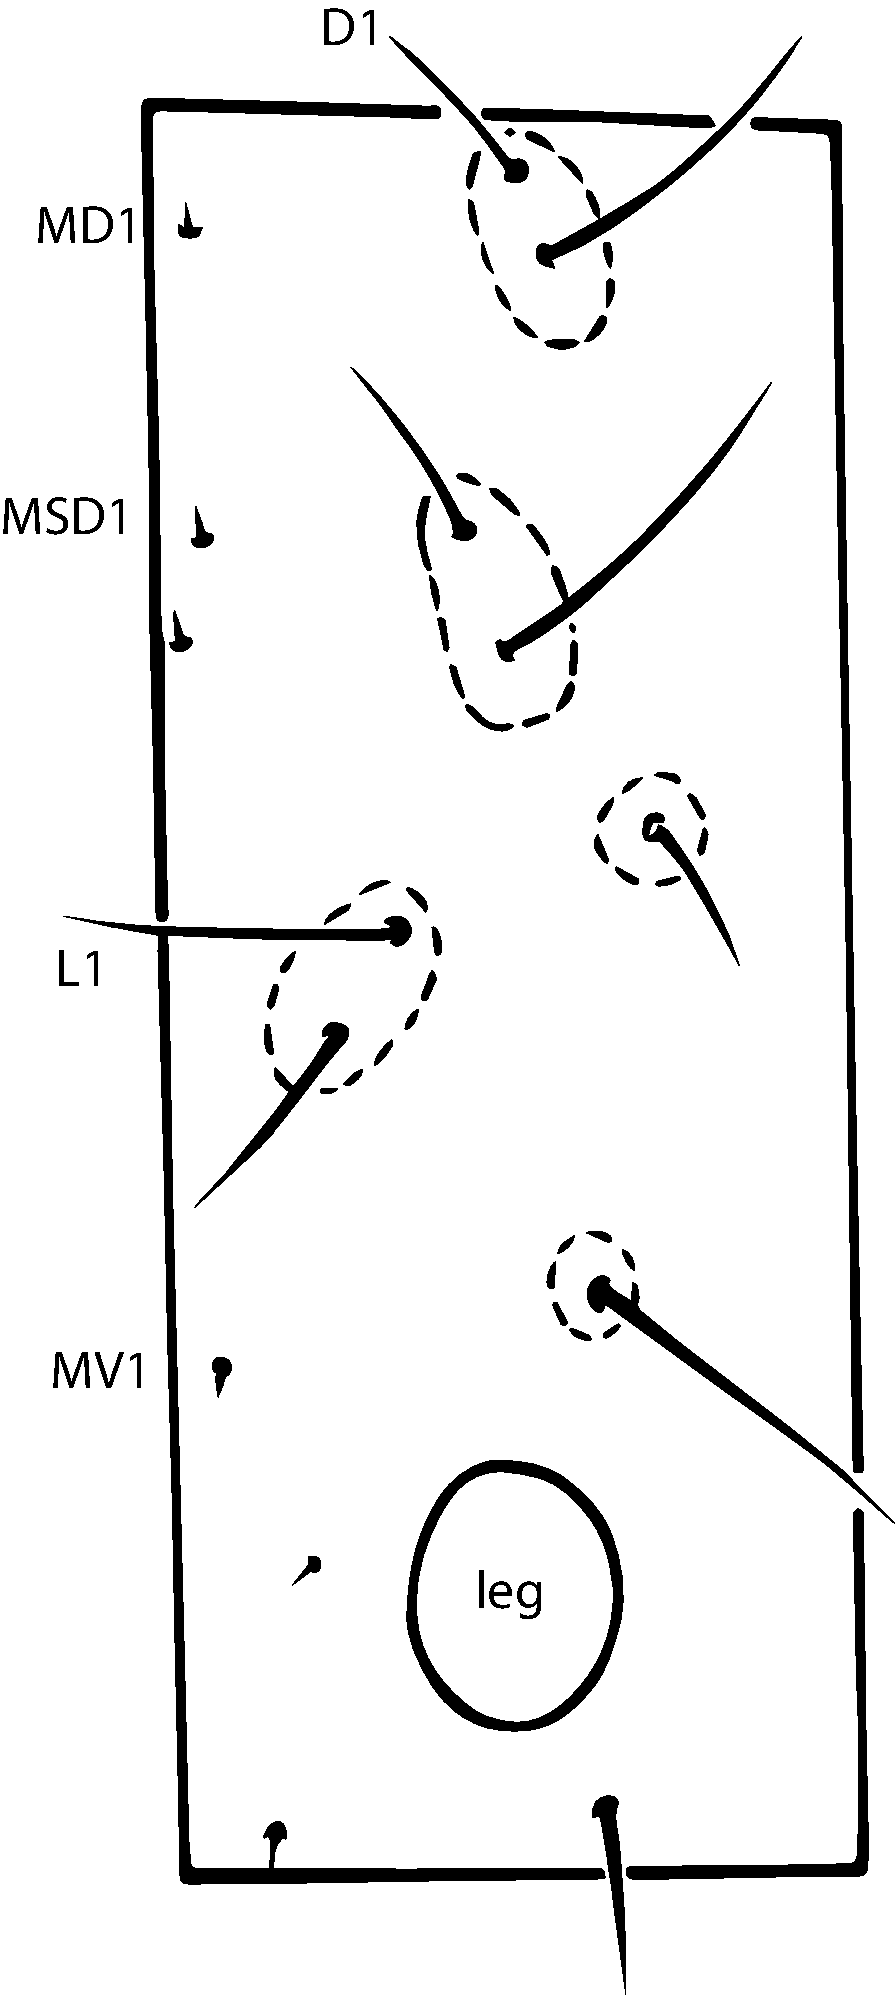
\includegraphics[width=\textwidth]{larvae/thoraxChaeto}
        \caption{thoracic segment}
        \label{fig:thoraxchaeto}
    \end{subfigure}
    \caption{\textbf{(a)} Chaetotaxy of the head capsule (Lepidoptera) \citep[redrawn and modified from][Fig. 26.1]{stehr1987immature}; \textbf{(b)} Chaetotaxy of a thoracic segment (Lepidoptera) \citep[redrawn and modified from][Fig. 26.21]{stehr1987immature}}\label{fig:chaeto}
\end{figure}%fair use? modified and redrawn

\section{Pupae}%https://doi-org.ezaccess.libraries.psu.edu/10.1016/B978-0-12-374144-8.00225-3
Transitioning from one form (larva) into another, often radically different form (adult) requires that the insect deconstruct and rebuild its body. This transition happens during a usually quiescent stage called the \latinword{pupa}. Pupae can take many forms, usually related to the position of their appendages, which are described below.

\subsection{Exarate}
\noindent{}\textit{Basic form:} Appendages stick out from the body (figures \ref{fig:exarate}, \ref{fig:decticous}). These pupae are not usually enclosed in a cocoon; some of these pupae are mobile.\vspace{3mm}

\noindent{}\textit{Example taxa:} Neuropterida, Trichoptera, some Lepidoptera, most Coleoptera\vspace{3mm}

\begin{figure}[ht!]
  \centering
    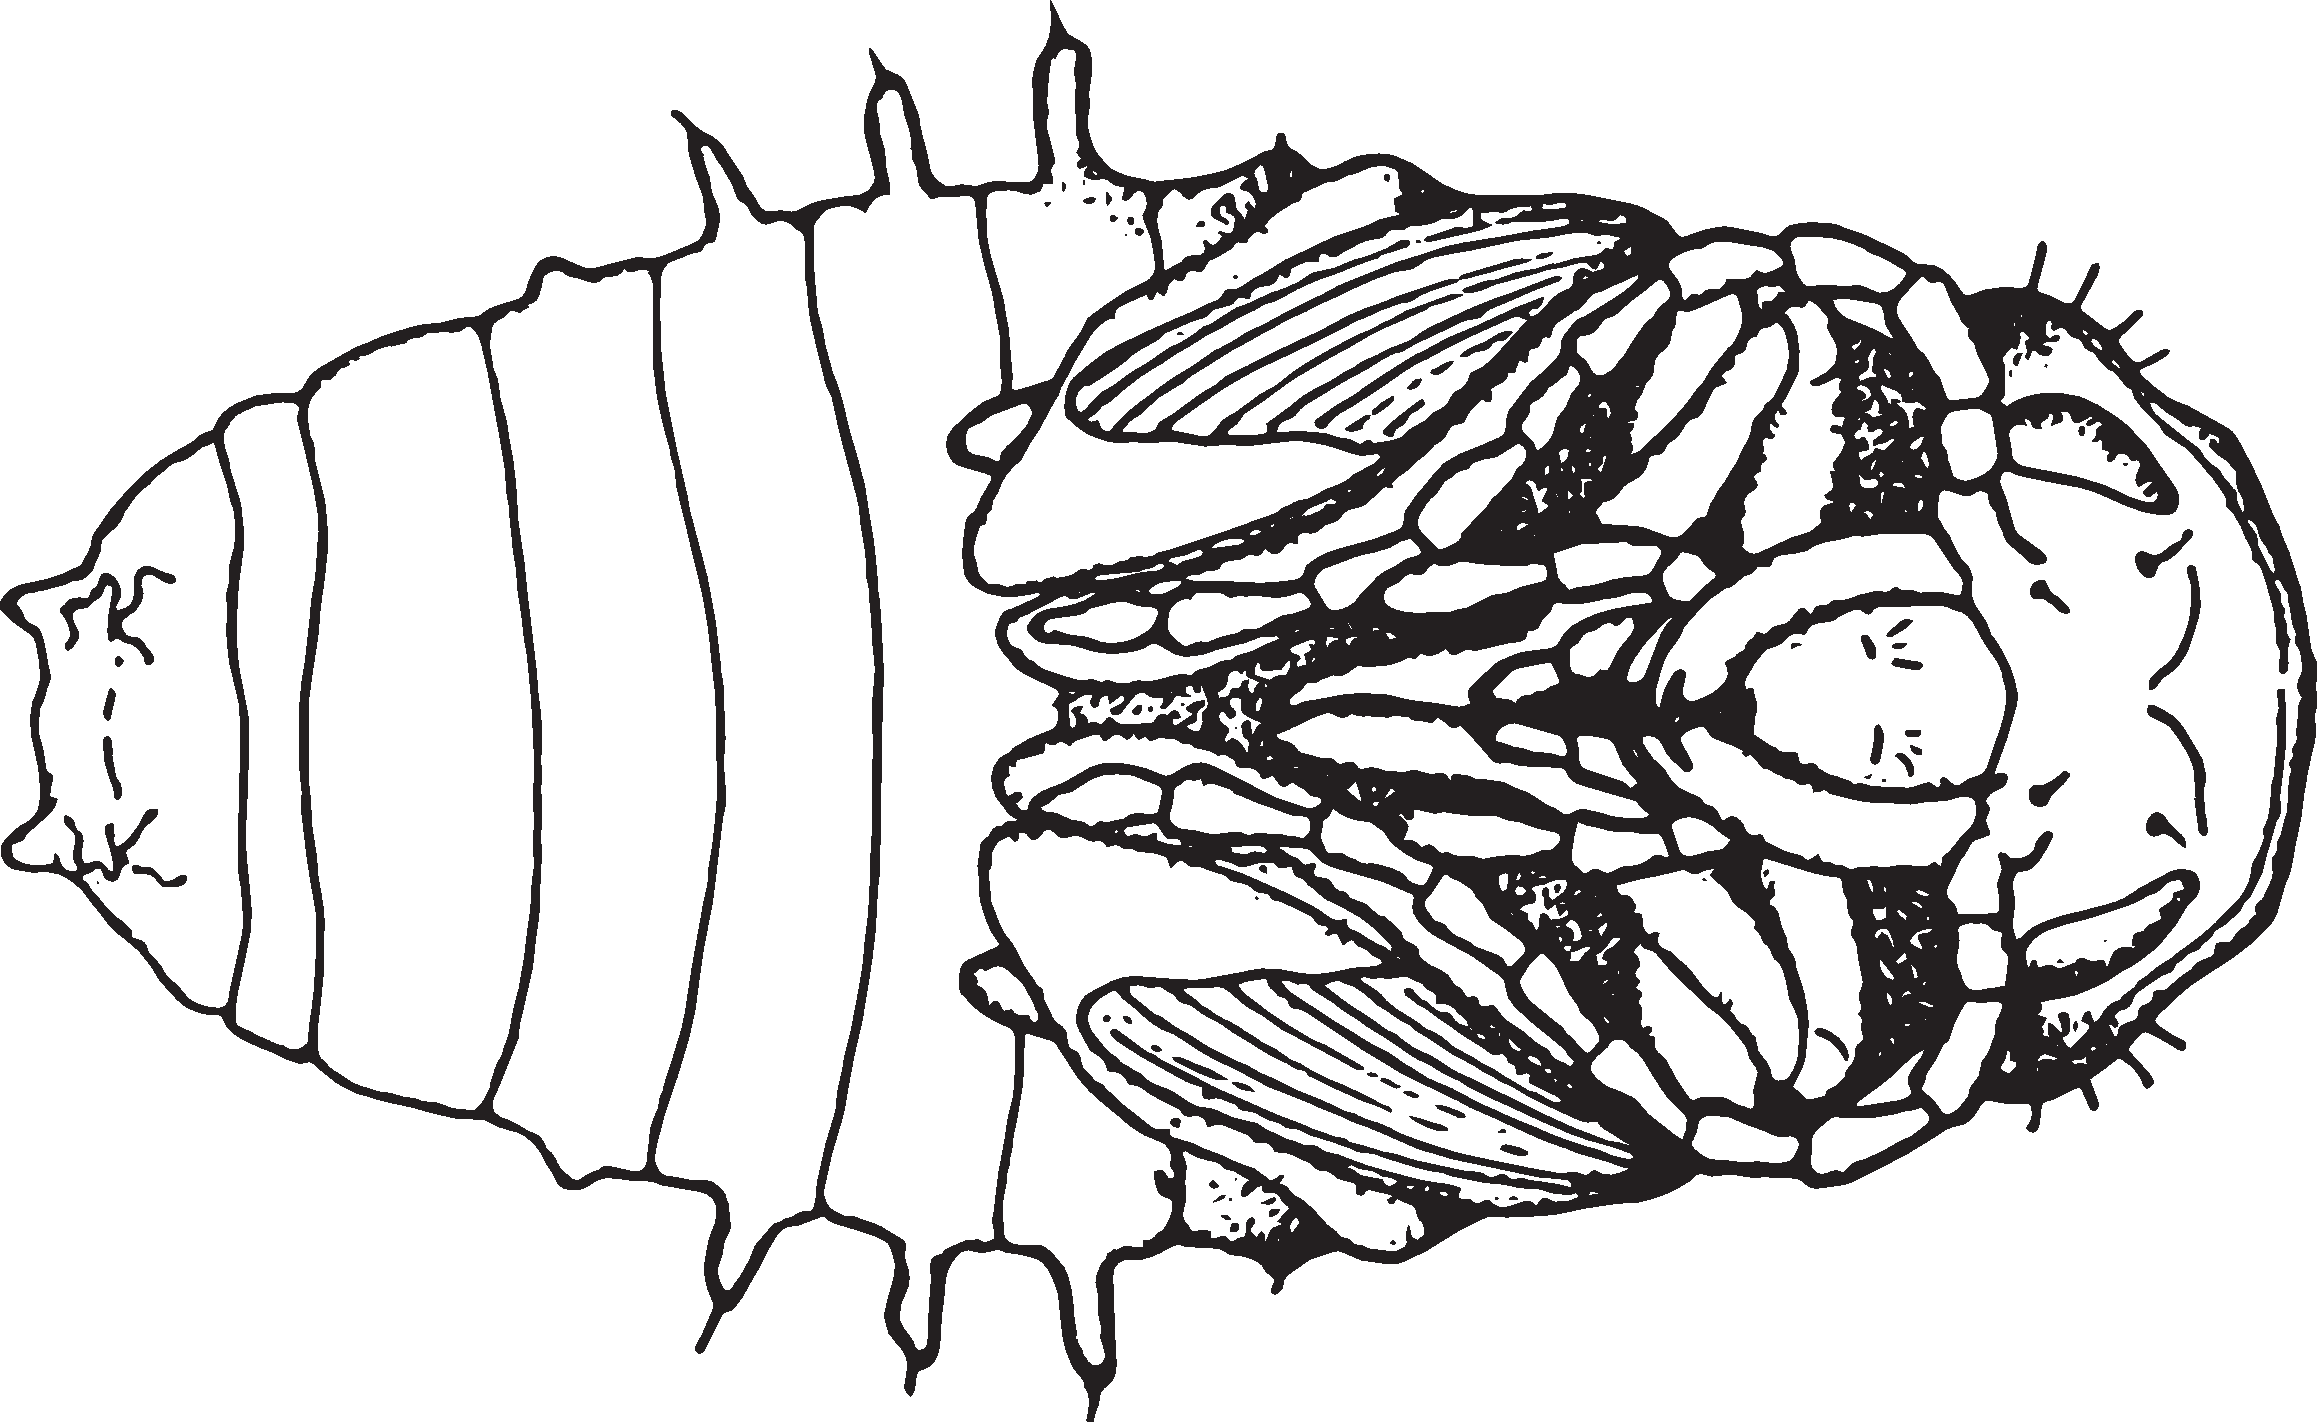
\includegraphics[width=0.5\textwidth]{larvae/exarate}
  \caption{Exarate pupa (Coleoptera) \citep[redrawn from][Fig. 2]{bhlpart193556}}
  \label{fig:exarate}
\end{figure}

\subsection{Obtect}% https://flic.kr/p/2kEAN8k
\noindent{}\textit{Basic form:} Appendages attached close to the body (figure \ref{fig:obtectAdecticous}),. These pupae are often protected by a silken cocoon.\vspace{3mm}

\noindent{}\textit{Example taxa:} Most Lepidoptera, Hymenoptera\vspace{3mm}

\begin{figure}[ht!]
  \centering
    \includegraphics[width=0.6\textwidth]{larvae/obtectAdecticous}
  \caption{Obtect, adecticous pupa (Lepidoptera) \citep[modified from][Fig. 6C]{bhlitem190298gelechiid}}
  \label{fig:obtectAdecticous}
\end{figure}

\subsection{Decticous}
\noindent{}\textit{Basic form:} These pupae have articulated mandibles (figure \ref{fig:decticous}), which usually function to break the adult insect free from the pupa.\vspace{3mm}

\noindent{}\textit{Example taxa:} Neuropterida, Trichoptera, some non-Ditrysia Lepidoptera\vspace{3mm}

\begin{figure}[ht!]
  \centering
    \includegraphics[width=0.6\textwidth]{larvae/decticous}
  \caption{Exarate, decticous pupa (Megaloptera) \citep[modified from][Fig. 56b]{walsh2004hellgrammite}}
  \label{fig:decticous}
\end{figure}

\subsection{Adecticous}
\noindent{}\textit{Basic form:} These pupae do not have articulated mandibles (figure \ref{fig:obtectAdecticous}).\vspace{3mm}

\noindent{}\textit{Example taxa:} Most holometabolous insects\vspace{3mm}

\subsection{Chrysalis}% https://flic.kr/p/2m85j5v ... https://flic.kr/p/2kM6bpD
\noindent{}\textit{Basic form:} Specialized obtect, adecticuous pupa, attached to the substrate via a velcro-like apparatus, between silken pad and pupal hooks (cremaster) (figure \ref{fig:chrysalis}). A belt-like structure, the girdle, attaches the middle of the pupa to the substrate.\vspace{3mm}

\noindent{}\textit{Example taxa:} Papilionoidea (butterflies)\vspace{3mm}

\subsection{Puparium (coarctate)}
\noindent{}\textit{Basic form:} The pupa is enclosed in the hardened cuticle of the penultimate larval instar (figure \ref{fig:puparium}).\vspace{3mm}

\noindent{}\textit{Example taxa:} Strepsiptera, many Diptera\vspace{3mm}

\begin{figure}[ht!]
    \centering
    \begin{subfigure}[ht!]{0.4\textwidth}
      \centering
        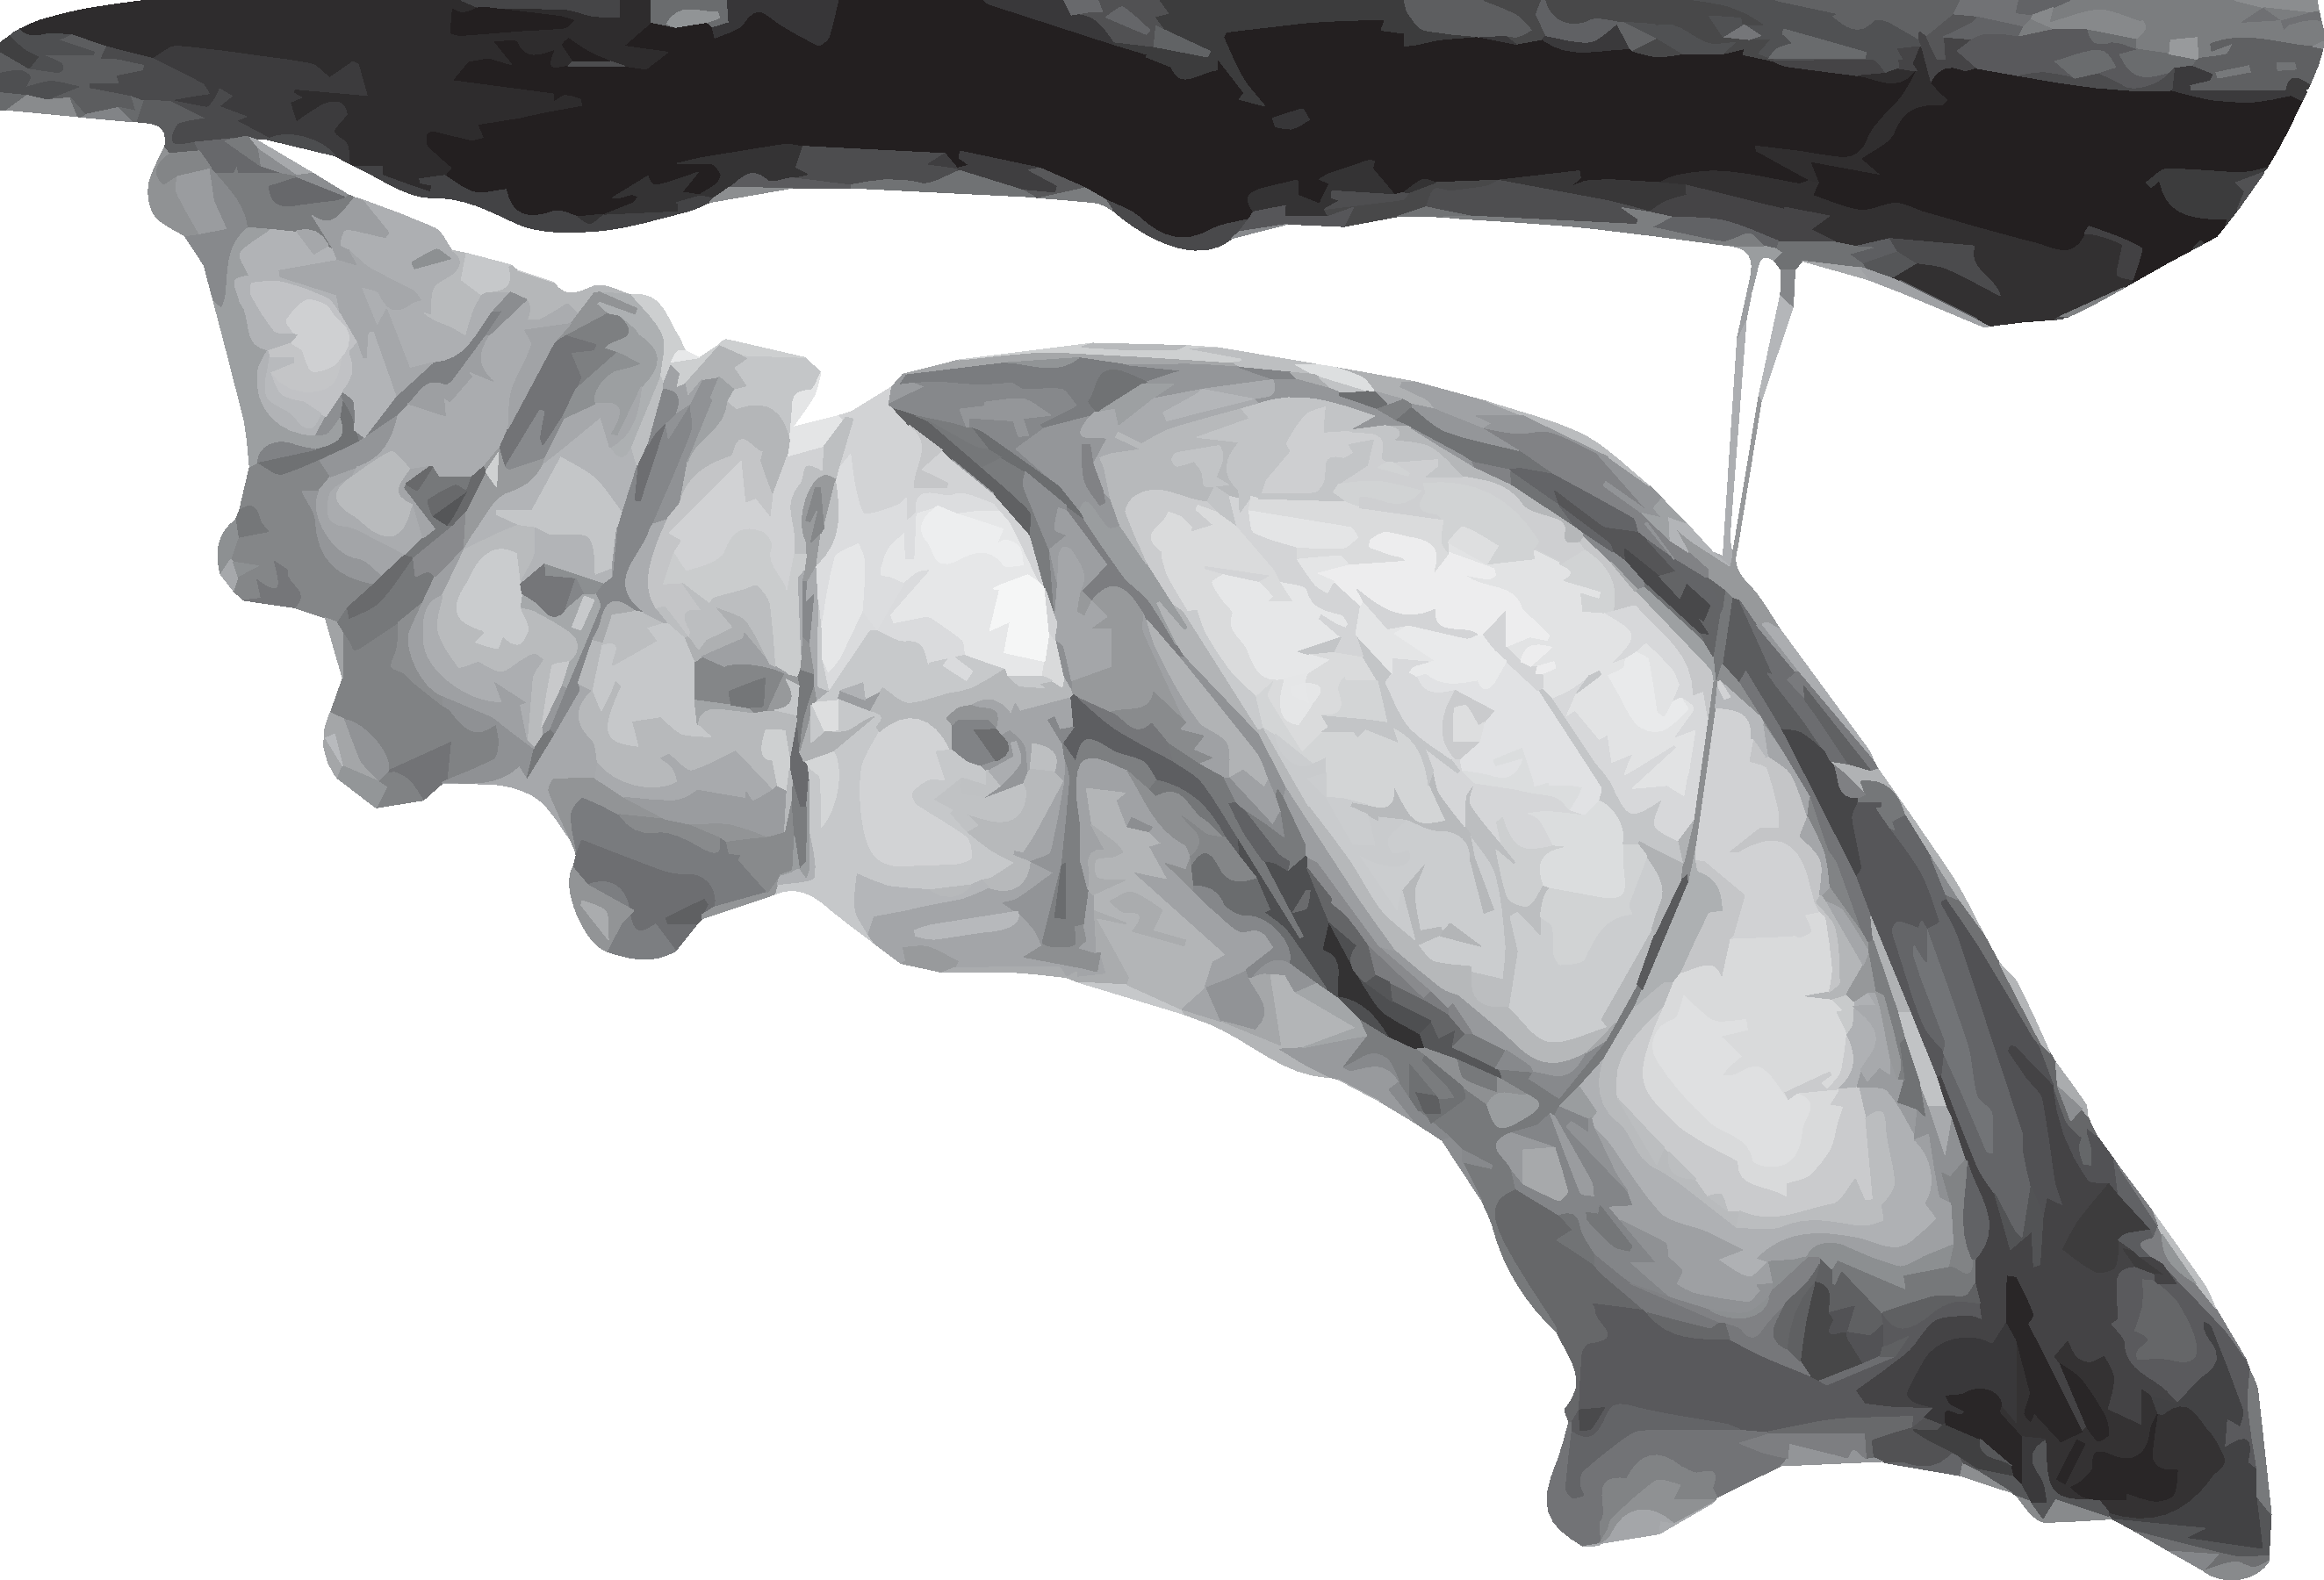
\includegraphics[width=\textwidth]{larvae/chrysalis}
        \caption{chrysalis}
        \label{fig:chrysalis}
    \end{subfigure}
    \hfill
    \begin{subfigure}[ht!]{0.45\textwidth}
        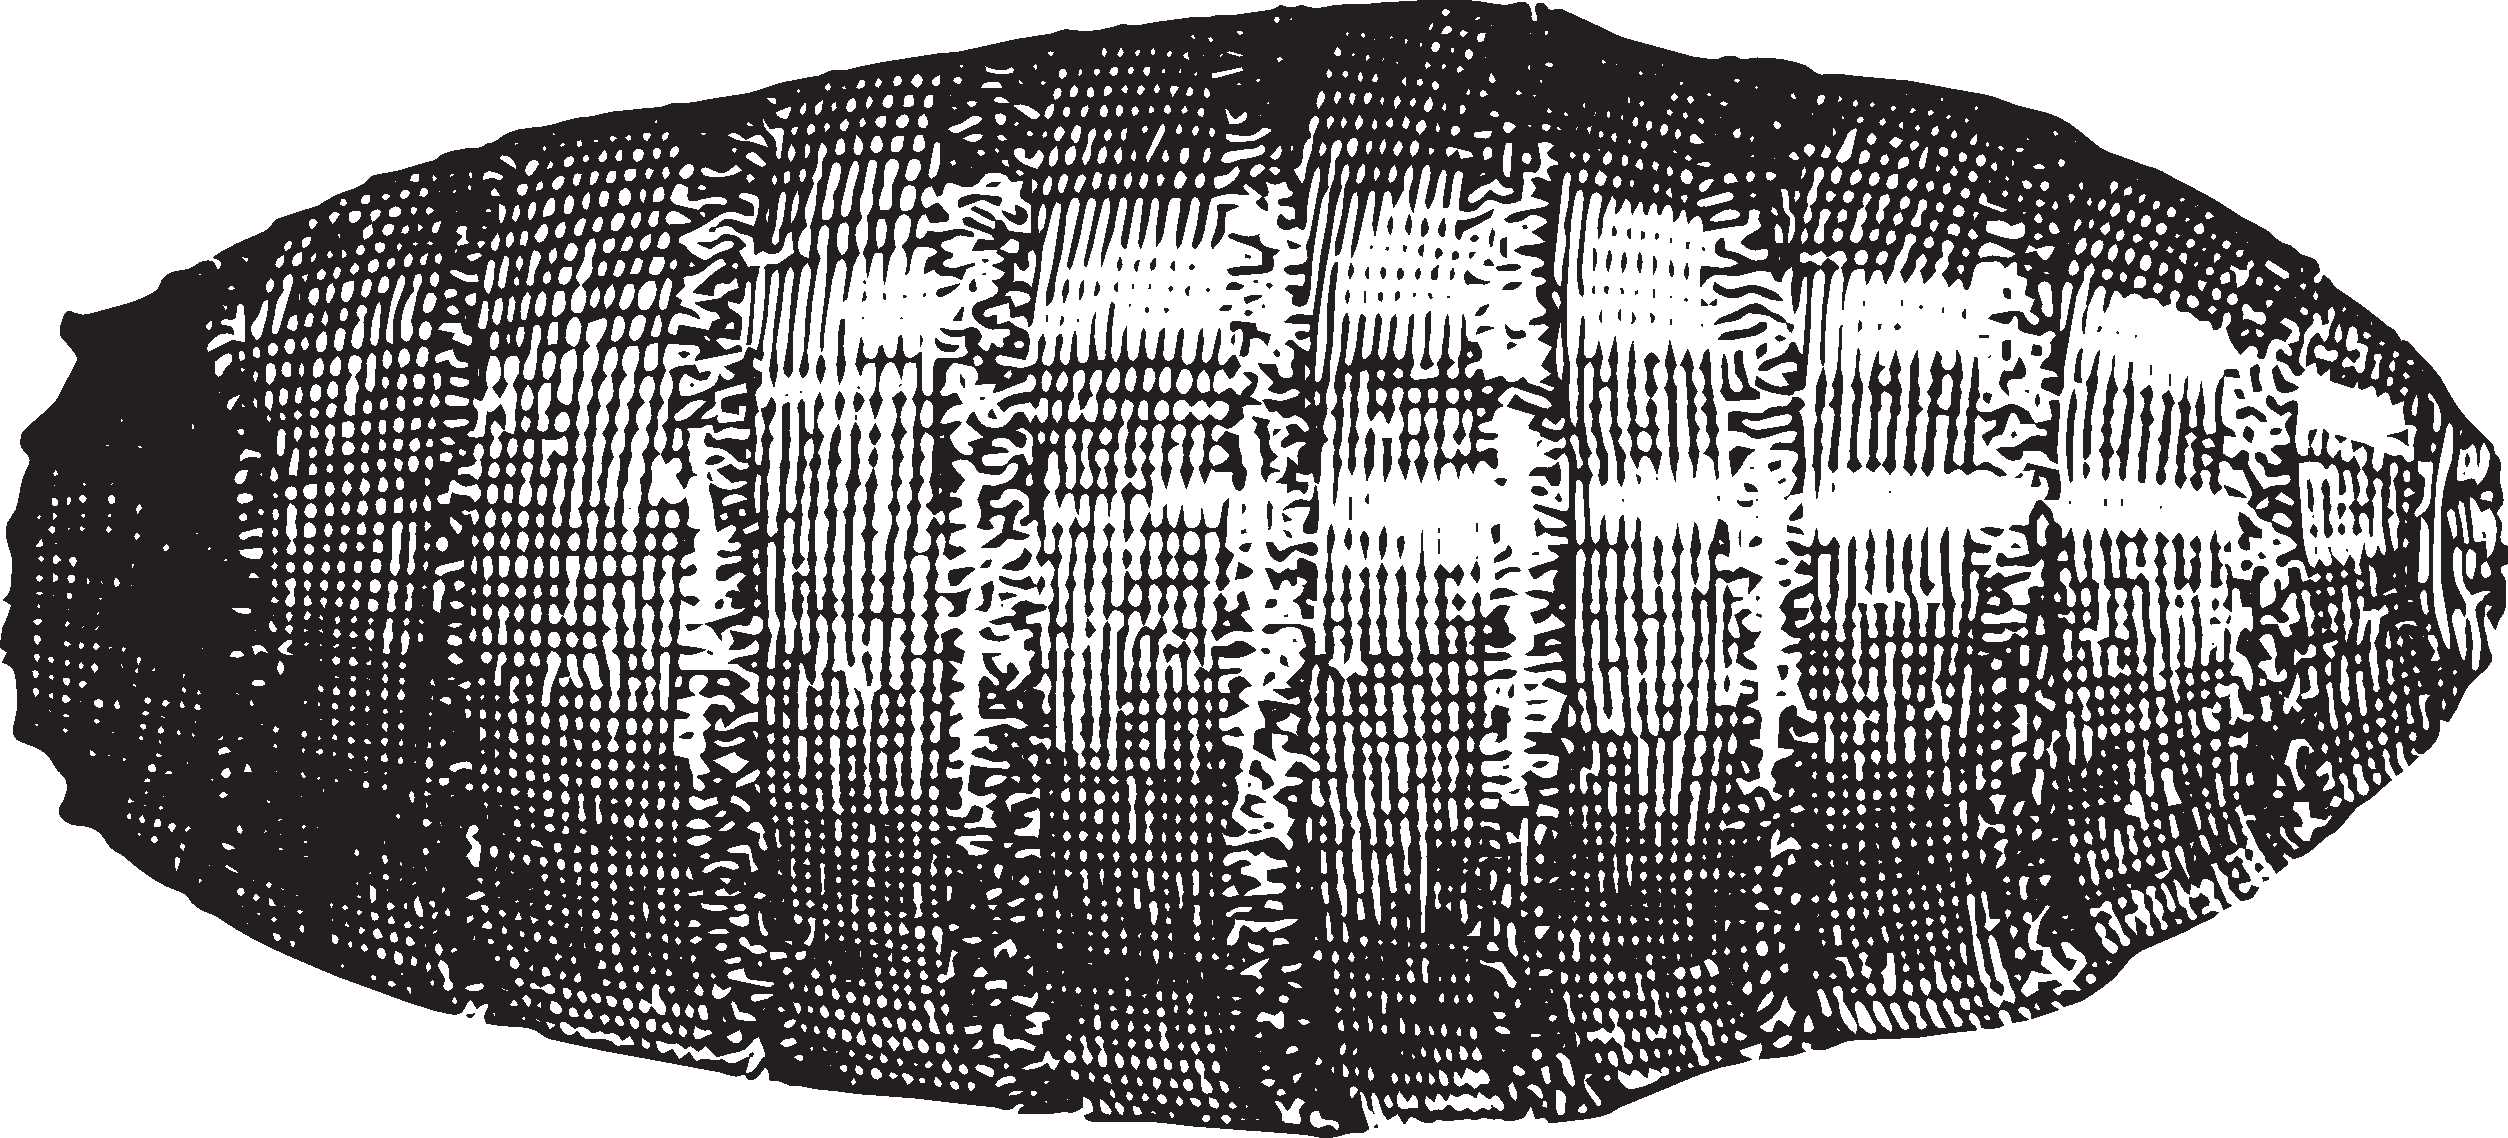
\includegraphics[width=\textwidth]{larvae/puparium}
        \caption{puparium}
        \label{fig:puparium}
    \end{subfigure}
    \caption{\textbf{(a)} Chrysalis (Papilionoidea). Digital drawing of photo by Patrick Coin (CC BY-NC-SA) \url{https://flic.kr/p/5cGLRs}; \textbf{(b)} puparium (Cyclorrhapha) \citep[redrawn from][Plate XXX, Fig. 5]{bhlitem82061AustrInsect}}\label{fig:pupae123}
\end{figure}

\begin{theo}
{}Can you explain the adaptive nature of the girdle and cremaster in the chrysalis?\vspace{3mm}

\noindent{}Why would the encasement of the pupa inside exuviae be advantageous for certain flies?
\end{theo}

\clearpage
\thispagestyle{empty}